\chapter{Estado del arte}\label{estadoarte}

En este capítulo se describirán los fundamentos teóricos y tecnológicos del proyecto. En primer lugar se presentará 
la identificación de tráfico y las distintas técnicas que existen para ello. También se explicará Bro \cite{broindex}, el 
sistema de monitorización de tráfico que se usará para llevar a cabo el desarrollo del proyecto. Así, se explicará su funcionamiento 
y, especialmente, el lenguaje de programación incorporado, analizándose cómo gestiona los eventos y sus funcionalidades básicas, así 
como la posibilidad de ampliar estas.

\intro Por último, se presentará de forma teórica en que consiste el emparejamiento de flujos y de qué forma se podría usar para 
identificar el tráfico.

\section{Identificación de tráfico}

Una definición de identificación de tráfico podría ser la siguiente, ``la clasificación del tráfico implica la asignación de objetos 
de tráfico a las clases de tráfico que los generan. La identificación usa terminología similar a la clasificación de tráfico. El 
término identificación se suele usar cuando se realiza de forma granular", cita de \cite{khalife2014}. Por lo que, se usará tanto 
identificación como clasificación indistintamente en las explicaciones de esta memoria.

\intro Esta técnica es usada para realizar muchas tareas de gestión y seguridad de la red. Como por ejemplo medidas de seguridad, 
garantizar la calidad de servicio \cite{microqos} e ingeniería de tráfico \cite{khalife2016}.

\subsection{Técnicas de identificación de tráfico}

Existen distintas técnicas para la identificación de tráfico, siendo distintas en función del nivel de granularidad que se aplique en 
el análisis \cite{khalife2016}. Existen tres grupos, los cuales se presentarán de forma breve.

\begin{itemize}
\item \textit{Paquetes}. Se realiza el análisis a los paquetes de forma individual.
\item \textit{Flujos}. Se analizan los flujos a partir de ciertos parámetros.
\item \textit{Host}. Se identifican las aplicaciones que usan los distintos equipos de la red.
\end{itemize}

\intro La más usada es la identificación basada en flujos, que es la que se utilizará en este trabajo.

\subsection{Identificación de tráfico basada en flujos}

En esta técnica, los flujos se analizan individualmente, pudiéndose dar un análisis global de la conexión o solamente de algunos de 
los paquetes que componen al flujo.

\intro Existen tres técnicas básicas de identificación de tráfico basada en flujos.

\begin{itemize}
\item Por los puertos de la capa de transporte, establecido por \textit{IANA} \cite{iana}.
\item Por el contenido del paquete o \textit{DPI} \cite{payload}.
\item Por la aplicación de técnicas de aprendizaje automático sobre estadísticas de tráfico, \textit{machine learning} 
\cite{learning}.
\end{itemize}

\intro Estas técnicas serán explicadas de forma más extensa a continuación.

\subsubsection{Identificación basada en puertos}

Esta técnica se basa en identificar el tráfico dependiendo de los puertos de la capa de transporte, según la asignación estándar 
de IANA \cite{ianaexplicacion}. 

\intro Por lo tanto, IANA es quien asigna el número de puerto oficial a los distintos protocolos, haciendo que, a priori, pueda 
identificar el tráfico por el número de puerto del servidor. 

\intro Esta técnica es la más simple y funcionaba correctamente, pero actualmente no es la más fiable. Esto se debe a la ofuscación de 
puertos, la multiplexación de puertos por diferentes servicios y el uso de otros puertos no oficiales.

\intro Un ejemplo de multiplexación de puertos podría ser el siguiente. En la actualidad, se están desarrollando multitud de 
aplicaciones web. Estas aplicaciones se conectan mediante el puerto 80, es decir, mediante el protocolo HTTP. Pero esto es solo 
teoría, pues se puede hacer que cualquier aplicación envíe información por el puerto 80, sin que pertenezca realmente a HTTP, lo cual 
daría como resultado una mala identificación.

\subsubsection{Aprendizaje automático}

En esta técnica de identificación, se hace uso de clasificadores basados en algoritmos de aprendizaje automático \cite{learning}. Se 
trata de un campo de investigación muy activo actualmente. En estas investigaciones se han propuesto y evaluado múltiples sistemas 
basados en distintos tipos de clasificadores, como redes neuronales, redes bayesianas o lógica fuzzy.

\intro A pesar de ser un campo de investigación muy actual y en el cual los métodos implementados son cada vez más inteligentes, los 
resultados no son buenos. Son costosos computacionalmente y al necesitar tiempo para el aprendizaje, se dan muchos errores en la 
clasificación.

\subsubsection{DPI}

La Inspección Profunda de Paquetes, DPI por sus siglas en inglés, \textit{Deep Packet Inspection}, realiza un análisis de los 
paquetes, entrando en el \textit{payload}, en busca de cadenas que permitan identificar de manera inequívoca el protocolo 
\cite{payload}. Dichas cadenas podrían ser \textit{GET} o \textit{POST} para el protocolo \textit{HTTP}, por ejemplo.

\intro Esta técnica suele ser usada por los proveedores de servicios de Internet, ISP, \textit{Internet Service Provider} y grandes 
empresas. Se puede decir que es una técnica que no respeta la privacidad, pues analiza la información contenida en el paquete. Aunque 
en el caso de una gran empresa si puede hacerse, pues si se está en la red propia no es delito mirar la información que contienen los 
paquetes.

\intro A pesar de ser la más efectiva en la actualidad, con una buena tasa de identificación y pocos errores \cite{dpiaproximacion}, 
presenta problemas a nivel de escalabilidad, al tener que analizar todos los paquetes de forma individual, y de privacidad, al entrar 
dentro de los paquetes, pudiendo llegar a ser ilegal en algunos países.

\section{BRO}

Bro \cite{broindex}, es un analizador de tráfico de red de código abierto, por lo que puede ser usado por quien lo desee 
sin necesidad de pagar licencias. Funciona sobre sistemas basados en Linux y Mac OS X \cite{brodownload}. Una de sus principales 
características es la gran cantidad de información que puede extraer con un solo escaneo. Otros monitores de red proporcionan menos 
información, teniendo que ser el propio administrador el que analice después la información obtenida por estos. Por lo tanto, tardará 
más en resolver los posibles problemas que encuentre en la red.

\begin{figure}[H]
  
\includegraphics[width=0.25\textwidth]{imagenes/logo-bro.png}
  \centering
  \caption{Logo de Bro.}
\end{figure}

\intro No tiene interfaz gráfica, por lo que su gestión se realiza desde la línea de comandos. Cuando se analiza 
tráfico, Bro generará unos registros con la información obtenida, los cuales están divididos en función de parámetros definidos por 
el equipo de desarrollo.

\intro Bro incorpora la posibilidad de introducir funcionalidades nuevas, mediante la programación en su 
propio lenguaje de \textit{scripting}, del mismo nombre. Esto se expondrá más adelante y, en el capítulo \ref{implementacion}, se 
mostrará cómo se desarrolla y algunos ejemplos de código escrito en Bro.

\intro El lenguaje de \textit{scripting} está orientado a trabajar con eventos. Por lo tanto, a la hora de añadir una nueva 
funcionalidad habrá que crearla a partir del uso de los eventos que puede gestionar el programa.

\intro Bro está estructurado de forma que todos los flujos de paquetes que analiza son procesados por el motor de eventos, 
como se puede ver en la Figura \ref{fig.arquitec}. Este motor convierte los flujos de paquetes en procesos de alto nivel, de forma que 
es más sencillo trabajar con ellos. Una vez que estos son tratados se generan los registros correspondientes, los cuales 
podrán ser analizados posteriormente \cite{broarquitectura}.

\begin{figure}[H]
  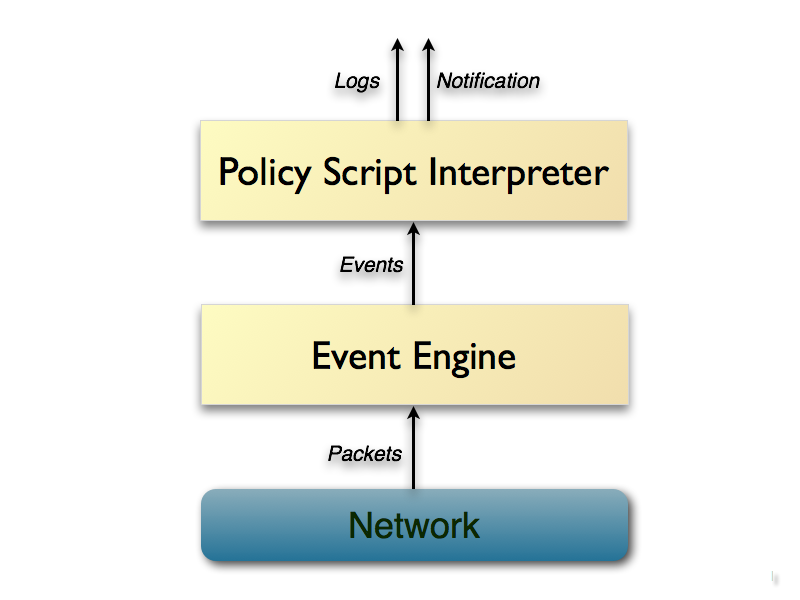
\includegraphics[width=0.7\textwidth]{imagenes/arquitectura-bro.png}
  \centering
  \caption{Arquitectura de Bro.}\label{fig.arquitec}
\end{figure}

\subsection{Funcionalidades básicas de BRO}

La funcionalidad básica de Bro es la monitorización de la red en la que se ejecuta. Mientras que se encuentra en ejecución, genera 
registros o \textit{logs} en texto plano que se podrán leer usando un editor de texto. Si se analiza un archivo \textit{pcap} los 
\textit{logs} no cambiarán tras finalizar el procesamiento. Sin embargo, si se analiza tráfico en tiempo real, los registros se irán 
actualizando a medida que pase el tiempo. Algunos de los \textit{logs} que se generarán son los siguientes.

\begin{itemize}
\item \textit{dpd.log}. Consiste en un resumen de los protocolos encontrados en puertos que no son estándar.
\item \textit{dns.log}. Contendrá toda la actividad correspondiente al \textit{DNS}
\item \textit{ftp.log}. Un registro de la actividad a nivel de sesión de \textit{FTP}.
\item \textit{files.log}. Un resumen con los archivos transferidos a través de una red. Incluye 
protocolos \textit{HTTP, FTP y SMTP.}
\item \textit{http.log}. Registro de toda la actividad \textit{HTTP} con sus respuestas.
\item \textit{ssl.log}. Un registro de las sesiones \textit{SSL}, incluidos los certificados que se utilizan.
\item \textit{weird.log}. En este \textit{log} se guarda la información correspondiente a actividad 
inesperada o rara a nivel de protocolo. Al analizar gran cantidad de tráfico no es muy útil, pues normalmente considera un volumen 
importante del tráfico como inesperado, pero a pequeña escala es bastante interesante para detectar, por ejemplo, intrusiones.
\item \textit{conn.log}. Aquí se puede ver la información correspondiente a sesiones \textit{TCP, UDP e ICMP}.
\end{itemize}

\intro Se puede consultar más información sobre \textit{logs} generados por una monitorización de Bro en \cite{brologs}.

\intro Bro dispone además de varios \textit{frameworks} que extienden su funcionalidad. Con ellos se podrán crear \textit{scripts} muy 
potentes. Algunas de las utilidades más relevantes son las siguientes.
\begin{itemize}
\item \textit{Geolocalización}. Se podrá encontrar la localización geográfica de una IP.
\item \textit{Análisis de ficheros}. El monitor de red tiene la capacidad de trabajar con ficheros.
\item \textit{Framework de loggins}. Con este \textit{framework} se podrá extender los archivos de registro que se generan.
\item \textit{NetControl}. Este \textit{framework} permitirá a Bro conectarse con distintos dispositivos de la red, como 
\textit{switches} o cortafuegos \cite{bronetcontrol}. En la Figura \ref{fig.netcontrol} se puede ver su arquitectura.
\begin{figure}[H]
  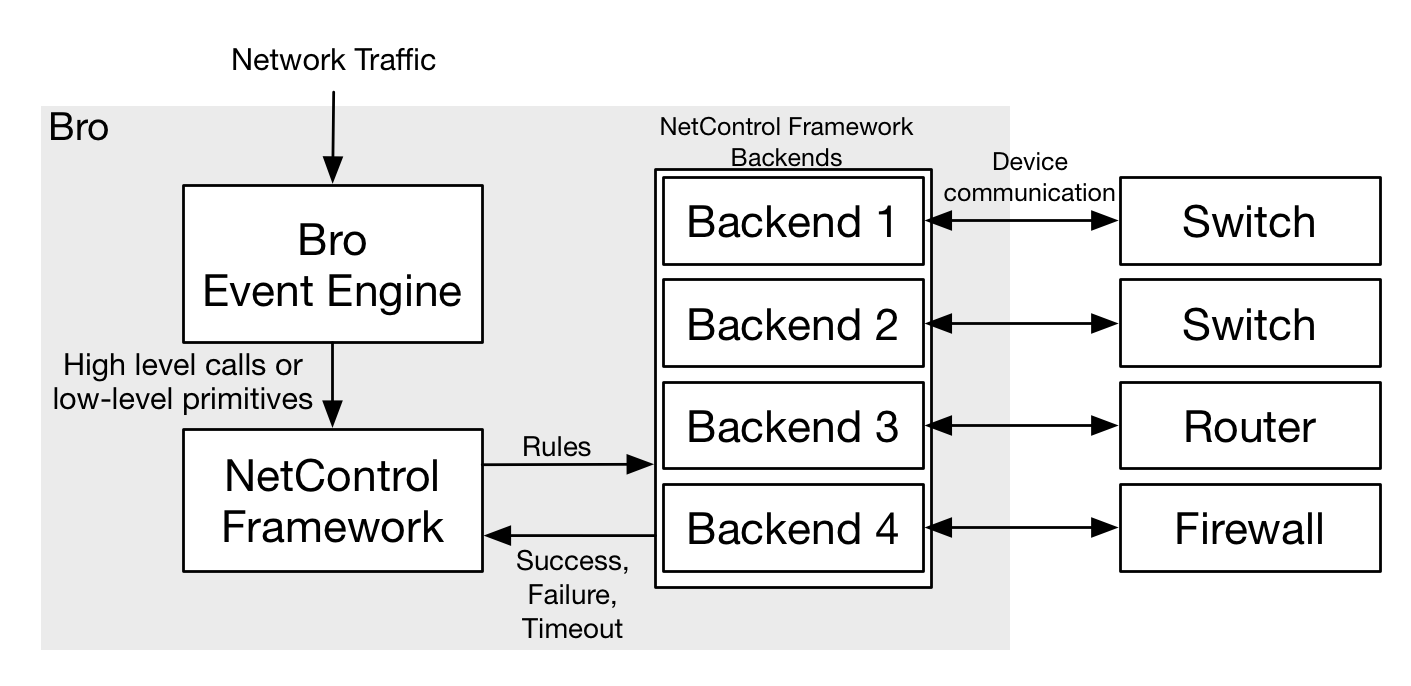
\includegraphics[width=0.9\textwidth]{imagenes/netcarquitectura.png}
  \centering
  \caption{Arquitectura de NetControl.}\label{fig.netcontrol}
\end{figure}
\end{itemize}

\intro Se pueden ver más detalles de estos \textit{frameworks} y otros en \cite{broframeworks}.

\intro A partir de la información de los registros, el administrador del sistema podrá determinar, entre otras cuestiones, si existen 
amenazas en la red o si hay algún componente defectuoso. Para ello deberá hacer uso de los eventos con los que Bro trabaja, para 
obtener un mayor conocimiento de todo el trabajo que se realice sobre la red.

\subsection{Eventos y trazas}

Aunque Bro permite la creación de funciones, la gestión e identificación del tráfico se realiza mediante eventos. Estos se dan cuando 
se detecta una determinada acción, por ejemplo, cuando detecta un paquete de respuesta \textit{UDP}, se activará el evento \textit{udp\_reply}.

\intro Dentro de cada evento se trabajará con la información del flujo que lo activa. Si captura información de una conexión 
\textit{TCP}, se tendrá que trabajar con ese tipo de flujo y las distintas variables globales que hayan sido definidas previamente.

\intro Para trabajar será necesario disponer de trazas de red, es decir, capturas de tráfico, que suelen estar en ficheros de formato 
\textit{pcap}. Se podrán obtener con un monitor de red, siendo en el caso de Bro necesario descargar un módulo adicional llamado 
\textit{trace-summary} \cite{brotrace}. Además de realizar capturas de tráfico, también da la posibilidad de separar el tráfico 
entrante del saliente, lo cual generará distintos registros. También se podrán conseguir distintas trazas de la web de Bro.

\intro De todo esto se obtiene que la programación de Bro esta orientada a eventos. Esto supone que no hay programación secuencial, 
por lo que se ejecutarán los distintos eventos según se vayan activando. Se tendrá que tener en cuenta los eventos que hay disponibles 
para detectar el distinto tipo de tráfico.

\subsection{Incorporación de funcionalidades}

La incorporación de funcionalidades al monitoreo realizado por Bro es una característica muy llamativa. Gracias 
a esto se podrá realizar un análisis muy personalizado usando un \textit{script} creado por el administrador de redes. De 
esta forma podrá, por ejemplo, filtrar el tráfico de una determinada IP mientras se sigue analizando el tráfico 
de forma normal, con los registros que genera Bro de forma automática. Es una forma muy sencilla de comprobar 
si por ejemplo el servicio que administra está recibiendo demasiadas peticiones desde una misma IP. Lo cual 
sería un indicio de ataque de denegación de servicio.

\intro A la hora de incorporar funcionalidades a Bro se puede hacer todo lo que se desee. Una búsqueda rápida 
por \textit{GitHub} arrojará una gran cantidad de personas que contribuyen con una gran cantidad de nuevas 
funcionalidades \citep{gitbeacon}. Ahora lo ideal sería incorporar un módulo, de forma que si el resto 
de la comunidad lo desea pueda hacer uso de él de una forma sencilla.

\section{Emparejamiento de flujos}\label{sec.emparejamiento}

La técnica de emparejamiento de flujos, fue planteada por investigadores del departamento de Teoría de la Señal, 
Telemática y Comunicaciones de la Universidad de Granada, en el año 2011 \cite{presentacion} \cite{comparacion}, para abordar 
los problemas de escalabilidad y privacidad de otras técnicas. Hay que tener en cuenta que el emparejamiento de flujos no es una 
técnica de identificación propiamente dicha, ya que no determina el tipo de flujo. Básicamente esta técnica lo que hace es agrupar los 
flujos de la misma clase, mediante asociaciones uno a uno.

\intro La idea de la que se parte es que dos flujos próximos en el tiempo, que comparten dirección IP y que usan números de puerto 
idénticos o próximos, deben de estar relacionados entre sí y corresponderán al mismo protocolo. 
Esto es, dos flujos que acceden al mismo servidor (IP) y puerto deberían de corresponder al mismo protocolo. Pero también dos flujos 
del mismo cliente con número de puerto consecutivos y muy próximos en el tiempo corresponderán, muy probablemente, al mismo protocolo 
y formarán parte de una secuencia de flujos de un interacción. 

\intro De esta forma, se define en \cite{comparacion} una función de similitud entre dos flujos a partir de las direcciones IP, los números de puerto y la proximidad temporal como se puede ver en la ecuación \ref{ecu}:

\begin{equation}\label{ecu}
	F(x,y)=
 	\begin{cases}
	  G(x,y), & N_{IP}(x,y) \geq 1 \\
	  -\infty, & \text{en otro caso}
	 \end{cases}
	 \addtocounter{neq}{1}
\end{equation}

\intro Donde G(x,y) es una función que evalúa la semejanza entre dos flujos, como se ve en \ref{ecug}:

\begin{equation}\label{ecug}
G(x,y) = |N_{IP}(x,y) – 1| + \frac{1}{dp1(x,y) + k1} + \frac{1}{dp2(x,y) + k1} + \frac{1}{dt(x,y) + k2}
\end{equation}

\intro Las variables de la función son las siguientes: 

\begin{itemize}
\item \textit{x, y}: Primer paquetes o flujos a comparar.
\item \textit{$N_{IP}(x,y)$}: Número de IP's coincidentes en ambos paquetes o flujos, estando el valor comprendido entre 0 y 2.
\item \textit{dp1(x,y)}: Se corresponde con la diferencia entre los números de los puertos de origen de los dos paquetes.
\item \textit{dp2(x,y)}: Será la diferencia entre los números de los puertos de destino de los dos paquetes.
\item \textit{k1, k2}: Son constantes que deben de ser estimadas experimentalmente. En \cite{comparacion} se proponen valores entre 1 
y 10000.
\item \textit{dt}: Es la diferencia de tiempo existente entre los tiempos de inicio de los flujos (\textit{timestamps}).
\end{itemize}

\intro El emparejamiento se realiza a partir del valor de similitud obtenido mediante la comparación con un umbral, que debe ser 
ajustado experimentalmente. Si se intentan emparejar todos los flujos mediante un umbral bajo, se producirán muchos errores, esto es, 
habrá una tendencia a que se consideren iguales flujos que no lo son, ya que pasarán el corte del umbral.

\intro Como se ha mencionado, el emparejamiento de flujos, por si mismo, no identifica el tráfico. Por lo tanto se 
necesitará otra técnica para clasificar el tráfico.
